\documentclass[11pt,a4paper]{article}

\usepackage[T1]{fontenc}
\usepackage[utf8]{inputenc}
\usepackage[margin=2.5cm]{geometry}
\usepackage{amsmath,amssymb}
\usepackage{booktabs,tabularx,array}
\usepackage{graphicx}
\usepackage{microtype}
\usepackage[numbers,sort&compress]{natbib}
\usepackage{xcolor}
\usepackage{placeins}
\usepackage[hidelinks]{hyperref}


\newcommand{\todo}[1]{\par\smallskip\noindent\textcolor{red!65!black}{\textbf{TODO:} #1}\par\smallskip}
\newcolumntype{Y}{>{\raggedright\arraybackslash}X}
\setlength{\emergencystretch}{2em}
\setlength{\parindent}{0pt}
\setlength{\parskip}{0.65em}

\title{Deep Reinforcement Learning for Bomberman}
\author{\texttt{Eric Flämig, Mark Salzmann, Jesper Eggers}}
\date{\today}

\begin{document}
\maketitle

\begin{abstract}
Bomberman combines navigation, delayed rewards, and decisions that can place
the agent itself in danger. 
This report discusses the two agents we developed parallely, both relying on the Double Deep Q-Network (Double DQN) learning algorithm.
\end{abstract}

\section{Theoretical Background and Agent Architecture}
\label{sec:theory}

\subsection{Bomberman as a reinforcement learning problem}
At each time step, the agent observes the game, chooses an action, and receives
feedback through game events. Its action set is
\[
\mathcal{A}=\{\texttt{UP}, \texttt{RIGHT}, \texttt{DOWN}, \texttt{LEFT}, \texttt{WAIT},\texttt{BOMB}\}.
\]
An episode corresponds to a round of play from the agent's perspective and
ends when it dies or the round terminates. The configured board has
$17\times17$ tiles, with a maximum of four agents and 400 steps per round.
The aim of the game is to collect coins and eliminate opponents. Coins yield points immediately, whereas placing a bomb can produce a benefit
only after its timer expires. The agent must therefore consider future
consequences rather than only the next reward.

The usual theoretical model is a Markov decision chain with states,
actions, transition probabilities, rewards, and discount factor $\gamma$.
The state of the game $s_t$ includes the positions of all agents, bomb timers, and revealed coins, as well as any other relevant game information needed to make decisions.
To make optimal decisions, the next action should be chosen based on the expected future rewards, considering both immediate and delayed consequences, captured by the action-value function defined as
\begin{equation}
Q^\pi(s,a)=\mathbb{E}_{\pi}\!\left[
\sum_{k=0}^{T-t-1}\gamma^k r_{t+k+1}
\,\middle|\,s_t=s,a_t=a\right].
\end{equation}
Here, $r_{t+1}$ is the learning reward, $T$ is the episode's terminal time,
and $\pi$ is the policy. A larger discount factor gives delayed outcomes
greater weight. For example, a useful bomb placement may deserve a high value
even if the agent must first move away and wait for the explosion.

\subsection{From Q-learning to deep Q-learning}
A deep Q-network (DQN) uses a neural network to approximate the action-value function, allowing it to generalize across similar states and handle large state spaces. 
For a given input state $s$ the network outputs a vector of action values $Q(s,a,\theta)$ for all possible actions $a \in \mathcal{A}$.

The learning process updates the network parameters $\theta$ using stochastic gradient descent

\begin{equation}
    \theta_{t+1} = \theta_t + \alpha\left(Y^Q_t - Q(S_t, A_t, \theta_t)\right) \nabla_\theta Q(S_t, A_t, \theta_t), 
\end{equation}
where $\alpha$ is the learning rate and $Y^Q_t$ is the target value for the Q-network at time step $t$ defined as
\begin{equation}
Y^Q_t = r_{t+1} + \gamma; \max_{a} Q(S_{t+1}, a, \theta_t).
\end{equation}

Previous steps get stored in the \emph{experience replay} buffer, which allows the network to sample minibatches of past transitions for training, reducing the correlation between consecutive updates.
Furthermore the target network with parameters $\theta^-$ is used to compute the target values, and it is updated every $\tau$ steps from the online network's parameters such that  $\theta^- = \theta_t$.
The target used in the update then becomes
\begin{equation}
Y^Q_t = r_{t+1} + \gamma \max_{a} Q(S_{t+1}, a, \theta^-),
\label{eq:dqn}
\end{equation}
where $\theta^-$ are the parameters of the target network.

\subsection{Double DQN: separating selection and evaluation}
The maximum in Equation~\eqref{eq:dqn} selects and evaluates an action using the same estimates. 
The issue with this method is that is prone to overstimation of action values, leading to bias in the learned Q-values.
Van Hasselt et al.\ show that this overestimation also occurs with deep networks and propose Double DQN to
reduce it \citep{vanhasselt2015double}.

They therefore propose the Double DQN approach, which uses the online network with parameters $\theta$ to select the next action and the target network with parameters $\theta '$ to evaluate that action.
These two networks are than updated independently, by assigning the change to either of the networks randomly during training. Important is that the changing the roles of the online and target networks is done in a symmetric manner.
The double DQN target is defined as
\begin{equation}
Y_t^{\mathrm{DoubleDQN}}=r_{t+1}+\gamma\;Q\Big(s_{t+1},\arg\max_{a}Q(s_{t+1},a, \theta_t);\theta'\Big),
\label{eq:double dqn}
\end{equation}
and note that action selection in the $\arg\max$ still uses the online parameter $\theta_t$. The best action of the greedy policy is still estimated using the current values, but the policy networks $\theta'$ is used to provide an unbiased evaluation of that action's value.

In Bomberman, a relevant motivation is to avoid overvaluing risky actions whose apparent payoff is based on inaccurate predictions.
The double DQN approach is beneficial in this context, as it helps the agent get more accurate value estimates for risky actions, leading to safer and more effective decision-making.

\subsection{Input representation and feature engineering}
The function \texttt{state\_to\_features} converts the observation into seven
spatial maps and ten scalar values. The board input has shape
$7\times17\times17$ and uses game information directly rather than rendered
screen pixels. Table~\ref{tab:2d-features} summarizes its channels.

\begin{table}[htbp]
\centering
\small
\begin{tabularx}{\textwidth}{@{}lY@{}}
\toprule
Channel & Encoding \\
\midrule
Walls & Binary map of indestructible walls. \\
Crates & Binary map of destructible crates. \\
Coins & Binary map of currently visible coins. \\
Bombs & Binary map of placed bomb locations. \\
Explosion map & Integer map of active explosions; the value represents the remaining duration. \\
Own position & Onehot encoding of the agent's tile\\
Opponents & Onehot encoding of each opponent's tile. \\
\bottomrule
\end{tabularx}
\caption{Spatial features implemented in \texttt{callbacks.py}.}
\label{tab:2d-features}
\end{table}

From these standard features, one can construct furher informative representations, such as combining bomb locations with the explosion map to a combined \texttt{danger map}.

The scalar input consits of the number of rounds, and steps played so far in the game.
Additionally it is useful for training to provide information about the agent's bomb availability, the number of remaining coins, the number of remaining opponents, the current step, and the previous action. Therefore we defined

\begin{table}[htbp]
\centering
\small
\begin{tabularx}{\textwidth}{@{}lY@{}}
\toprule
Channel & Encoding \\
\midrule
Bomb availability & Binary value indicating if the agent can place a bomb. \\
Number of coins normalised & Float32 value representing the number of all collectable coins divided by the total number of coins. \\
Number of opponents & Integer value representing the number of opponents. \\
Current step & Integer value representing the current step in the game. \\
Previous action & One-hot encoding of the previous action taken by the agent. \\
Own position & Onehot encoding of the agent's tile\\
Opponents & Onehot encoding of each opponent's tile. \\
\bottomrule
\end{tabularx}
\caption{Scalar features implemented in \texttt{callbacks.py}.}
\label{tab:scalar-features}
\end{table}

By providing the agent with absolute information about the game state, such as the number of remaining coins, opponents, and the current step, the network can make more informed decisions.


\subsection{Exploration with an epsilon-greedy policy}
The agent implements an $\epsilon$-greedy policy. Let $\mathcal{A}_m(s)$ be
the actions retained by its mask. During training, the action is sampled as
\begin{equation}
a_t=\begin{cases}
\text{a uniform random action from }\mathcal{A}_m(s_t),
& \text{with probability }\epsilon_t,\\
\displaystyle\operatorname*{arg\,max}_{a\in\mathcal{A}_m(s_t)}
Q_\theta(s_t,a), & \text{with probability }1-\epsilon_t.
\end{cases}
\end{equation}
Exploration supplies experience with actions that the current network may
undervalue, whereas exploitation uses what has already been learned. Both branches
respect the mask. The random branch can also select the greedy action, so
$\epsilon_t$ is the probability of random selection, not necessarily the
probability of taking a non-greedy action.

In order to provide sufficient exploration early in training, but gradually reduce it as the agent learns, we use an exponentially decaying epsilon
\begin{equation}
\epsilon_t=\epsilon_{\min}+
(\epsilon_{\mathrm{start}}-\epsilon_{\min}) \cdot \exp\left(-\frac{t}{T_{\mathrm{decay}}}\right).
\end{equation}
It is beneficial to choose $T_{\mathrm{decay}} = \frac{T_{\mathrm{Half-life}}}{\ln 2}$.

During the whole training process, the agent is faced with different training epochs. 
This introduces varying scenarios, obstacles, and opponents.
To provide adequate exploration, it is a good trick to reset epsilon to a middle value at the beginning of each new training epoch, as discussed in \ref{sec:curriculum}.


\subsection{Ruehl based agent}

\subsubsection{Neural network architecture}
Given the combination of spatial and scalar features, it is reasonable to use a network architecture that processes these two types of inputs separately before combining them for decision making.
The spatial branch contains four convolutional layers with ReLU activations.
Dilated convolutions expand the area visible to a filter without increasing its number of weights, while the third convolution reduces the spatial resolution. 
Table~\ref{tab:network} gives the dimensions derived from
\texttt{Networks.py} with the batch dimension is omitted.

\begin{table}[htbp]
\centering
\small
\begin{tabularx}{\textwidth}{@{}lYl@{}}
\toprule
Component & Operation & Output shape \\
\midrule
Board input & Seven spatial channels & $7\times17\times17$ \\
Convolution 1 & $3\times3$, 32 filters, stride 1, padding 1 & $32\times17\times17$ \\
Convolution 2 & $3\times3$, 32 filters, dilation 2, padding 2 & $32\times17\times17$ \\
Convolution 3 & $3\times3$, 32 filters, stride 2, padding 1 & $32\times9\times9$ \\
Convolution 4 & $3\times3$, 32 filters, dilation 2, padding 2 & $32\times9\times9$ \\
Flatten & Flatten the board features & $2592$ \\
Scalar branch & Linear $10\to32$, ReLU & $32$ \\
Concatenation & Join spatial and scalar features & $2624$ \\
Shared layers & Linear $2624\to128\to128$, ReLU after each & $128$ \\
Value head & Linear $128\to1$ & $1$ \\
Advantage head & Linear $128\to6$ & $6$ \\
\bottomrule
\end{tabularx}
\caption{Architecture of the RUEHL network for the configured board size.}
\label{tab:network}
\end{table}
Each output of the last convolution has a theoretical receptive field of $17\times17$ input tiles, including padding near the boundary. The flattened features subsequently connect to shared fully connected layers.

Complementing the double DQN strategy, one can employ a dueling network architecture to separately estimate state values and action advantages, which can lead to more stable learning and improved policy evaluation.
In the dueling DQN architecture, the action-value function is not represented directly by a single network output. Instead, the network decomposes the estimate of \(Q(s,a)\) into two components: a state-value function \(V_\theta(s)\) and an action-dependent advantage function \(A_\theta(s,a)\) \citep{wang2016dueling}. The state-value function represents the overall quality of being in state \(s\), independently of which action is selected, whereas the advantage function describes the relative benefit of choosing a particular action \(a\) in that state.

A naive decomposition of the form

$$
Q_\theta(s,a)=V_\theta(s)+A_\theta(s,a)
$$

is not identifiable. In particular, an arbitrary constant \(c\) can be added to the value function and subtracted from all advantage values without changing \(Q_\theta\):

$$
V_\theta(s)+c
+
\left(A_\theta(s,a)-c\right)
=
V_\theta(s)+A_\theta(s,a).
$$

Consequently, the network would have no unique way of determining which part of the predicted action value should be represented by \(V_\theta\) and which part should be represented by \(A_\theta\).

To remove this ambiguity, the dueling architecture combines the two streams by subtracting the mean advantage over all available actions,
\begin{equation}
Q_\theta(s,a)=V_\theta(s)+A_\theta(s,a)
-\frac{1}{|\mathcal{A}|}\sum_{b\in\mathcal{A}}A_\theta(s,b).
\label{eq:dueling}
\end{equation}
This centers the effective advantage values around zero. 
An important consequence of this parameterization is obtained by averaging \(Q_\theta(s,a)\) over all actions:

$$
\frac{1}{|\mathcal A|}
\sum_{a\in\mathcal A}Q_\theta(s,a)
=
V_\theta(s).
$$

Thus, under this aggregation rule, the value stream represents the mean predicted action value in a state, while the centered advantage stream determines how the individual action values differ from this common baseline. In particular, because both \(V_\theta(s)\) and \(\bar A_\theta(s)\) are independent of the selected action,

$$
\arg\max_{a} Q_\theta(s,a)
=
\arg\max_{a} A_\theta(s,a).
$$

Hence, the advantage stream determines the relative ranking of actions, whereas the value stream controls the overall level of their Q-values.

The motivation for this decomposition is that in many states the precise choice of action has only a small effect on the expected return. A conventional DQN must nevertheless estimate a separate \(Q(s,a)\) for every action. The dueling architecture allows the network to learn features that characterize whether a state is generally favorable or unfavorable through \(V_\theta(s)\), while using the advantage stream only to represent differences between actions. This can make value estimation more efficient in states where several actions have similar consequences \citep{wang2016dueling}.

The two quantities are not trained using separate value and advantage targets. Instead, they are combined according to Eq.~\eqref{eq:dueling} to obtain \(Q_\theta(s,a)\), and the usual temporal-difference loss is applied to this resulting Q-value. Gradients then propagate through the aggregation operation into both the value and advantage streams. The decomposition is therefore an architectural parameterization of the Q-function rather than the introduction of two independently supervised learning objectives.


\FloatBarrier



\subsubsection{Training curriculum} \label{sec:curriculum}
The training progression considered in this project starts with navigation,
then introduces bomb use, and finally adds opponents. This curriculum is
motivated by the difficulty of discovering all three behaviors at once:
an inexperienced agent can otherwise die before collecting useful examples
of delayed rewards. Table \ref{tab:curriculum} links the progression to the
available scenarios.

\begin{table}[htbp]
\centering
\small
\begin{tabularx}{\textwidth}{@{}lccY@{}}
\toprule
Scenario & Crate density & Coins & Role in the curriculum \\
\midrule
\texttt{coin-heaven} & $0$ & $50$ & Learn movement and collection; the initial stage is intended to run without opponents. \\
\texttt{loot-crate} & $0.75$ & $50$ & Learn to open routes, reveal coins, and escape after placing bombs. \\
\texttt{classic} & $0.75$ & $9$ & Combine collection and bomb use with competition against opponents. \\
\bottomrule
\end{tabularx}
\caption{Configured scenarios and their intended training roles. Crate
density is the placement probability before walls and starting areas are
cleared. Opponents are configured separately from the scenario.}
\label{tab:curriculum}
\end{table}

\paragraph{Stage 1: coin collection.}
In the \texttt{coin-heaven} scenario, visible coins give a relatively direct
objective: move through the maze and collect them efficiently. The agent can
learn spatial relationships between its position, walls, and rewards.
For this initial stage of training, we started the epsilon greedy strategy with $\epsilon = 1$, ensuring maximum exploration. 
Via reward shaping, the agent receives immediate feedback for collecting coins, and negative feedback for undesirable actions, guiding it towards efficient coin collection.

\paragraph{Stage 2: crate destruction.}
The \texttt{loot-crate} scenario adds destructible obstacles and places coins
preferentially underneath them. Successful collection can now require a
sequence of actions: approach a crate, place a bomb, reach safety, and return
to collect a revealed coin. This stage introduces delayed credit assignment
and the conflict between making progress and avoiding self-destruction.
Initializing from the pretrained Network on \texttt{coin-heaven}, we continued training with substantial epsilon reheating $\epsilon = 0.85$ to encourage exploration in the presence of destructible crates. 
For this stage, a different reward profile is used, emphasizing successful crate destruction and safe bomb placement, while still rewarding coin collection and very importantly, penalises suicidal actions.

\paragraph{Stage 3: opponents and competitive play.}
The main goal for this stage is to adapt to less placed coins, while dealing with dynamic opponents.
A progression from simpler opponents to stronger ones would let the agent adapt these skills gradually. 
For this purpose, we iteratively improved the model, by transfering the pretrained network from \texttt{loot-crate} to \texttt{classic} with slight epsilon reheating $\epsilon = 0.20$, then gradually increased the difficulty of opponents.


\subsubsection{Action masking and hand-designed guidance}
The mask is an important part of an effective policy. It first rejects
movement into walls, crates, bombs, or opponents. It then filters movement
and waiting on active explosions or blast tiles of bombs whose timers are
at most one. Bomb placement is allowed only when a bomb is available, its
blast could hit a crate or opponent, and a static breadth-first search finds
a tile outside its blast within the configured bomb timer.

If no action survives the danger filter, the code falls back to the earlier
legal-action mask. If that is also empty, the model chooses \texttt{WAIT}.
This is therefore a heuristic filter, not a guarantee of survival. 
Its static escape search does not predict moving opponents or jointly simulate other bombs over time.

This guidance reduces the exploration burden, but it also contributes to
the observed behavior independently of learned Q-values. Results should
therefore describe the complete network-plus-mask policy. The Double DQN
update in \texttt{train.py} also applies the next-state
action mask before the online network selects its maximizing action. The
target network then evaluates that selected action.

\subsubsection{Reward shaping}
\label{sec:reward-design}
The main goal of the agent is to maximize game score at the end of the game, by collecting coins, eliminating opponents, given by
\begin{equation}
S=N_{\mathrm{coins}}+5N_{\mathrm{opponents\ killed}}.
\end{equation}
However, starting from these sparse and delayed objectives alone makes it difficult for the agent to learn effective strategies.
Reward shaping addresses this problem, by giving intermediate rewards and punishments that guide the agent's behavior before the final game outcome is known.
For the \texttt{ruehl\_based\_agent}, we rejected anisotropic rewards, meaning rewards that vary depending on the direction or context of the action. 
Combined with the CNN architecture, this design choice ensures that the agent exploits the symmetry of the game environment.
Furthermore, we only introduce additional shaping rewards that are deductable from the input game state, e.g. rewarding the survival of own placed bombs or penalizing the agent for being in the blast radius of an active explosion.
Furthermore, one can differentiate between main rewards, connecting to significant game events, and shaping rewards, which serve as fine tuning of the agent's behavior. The shaping rewards are an order of magnitude smaller than the main rewards.

\paragraph{Main rewards}
The main contribution, stored under \texttt{major},
assigns values to selected game events.
Collecting a coin provides a baseline reward, typically 1 point, in accordance with the actual game score.
Other rewards will be scaled relative to this baseline.
A separate Self-destruction penalty is useful in competitive play. 
This expresses the trade-off between gaining points and retaining the opportunity to act. 
Penalizing only death would encourage excessive caution, meanwhile rewarding only attacks would provide insufficient feedback about their danger. 
Their combination is intended to encourage productive risks with an escape plan.

\paragraph{Shaping penalties}
The separate shaping terms discourage waiting, entering an active explosion,
and, in the competitive profile, immediately reversing movement direction.
Their purpose is to discourage inactivity and repeated back-and-forth motion
without making these actions impossible. Waiting for an explosion to clear
or reversing direction to escape can be necessary, so these penalties should
remain small relative to important outcomes.

\subsubsection{Task-specific reward profiles}
We identified three substantially different challenges, for which we designed corresponding reward profiles: \texttt{coin}, \texttt{loot\_exploration}, and \texttt{killer}. 
Determining the appropriate distribution of rewards was a challenging task that required long trial and error processes.
The current values are summarized in Table~\ref{tab:reward-profiles}.

\begin{table}[htbp]
\centering
\small
\begin{tabularx}{\textwidth}{@{}Yrrr@{}}
\toprule
Event or parameter & \texttt{coin} & \texttt{loot\_exploration} & \texttt{killer} \\
\midrule
Coin collected & $1.0$ & $1.0$ & $1.0$ \\
Coin revealed & $0.1$ & $0.5$ & $0.5$ \\
Crate destroyed & $0$ & $0.35$ & $0.15$ \\
Bomb placed to hit a crate & $0$ & $0.05$ & $0.02$ \\
Bomb placed to threaten an opponent & $0$ & $0$ & $0.75$ \\
Opponent killed & $6.5$ & $6.5$ & $6.0$ \\
Killed by another agent & $-1.0$ & $-1.0$ & $-2.0$ \\
Self-destruction & $-2.0$ & $-2.0$ & $-6.0$ \\
Bomb exploded & $0$ & $0$ & $0.15$ \\
Round survived & $0$ & $0$ & $0.75$ \\
\midrule
Waiting (shaping) & $-0.08$ & $-0.01$ & $-0.05$ \\
Danger (shaping) & $-0.02$ & $-0.04$ & $-0.10$ \\
Reversing direction (shaping) & $0$ & $0$ & $-0.03$ \\
Shaping limit $c$ & $0.05$ & $0.05$ & $0.15$ \\
Step cost $\lambda$ & $0.008$ & $0$ & $0.002$ \\
\bottomrule
\end{tabularx}
\caption{Reward profiles in \texttt{train.py}. Event values are summed per
transition; only the combined shaping contribution is clipped. A zero denotes
an event with no assigned reward in that profile.}
\label{tab:reward-profiles}
\end{table}

\paragraph{Coin collection.}
The \texttt{coin} profile rewards collection and discourages waiting through
both a shaping penalty and a small step cost. It gives no direct incentive
for crate destruction or bomb placement, focusing the initial task on
navigation. Opponent-kill rewards are inherited from the shared reward table
but have no effect in a scenario without opponents.

\paragraph{Crate exploration.}
The \texttt{loot\_exploration} profile rewards destroying crates, revealing
coins, and placing bombs whose blast reaches a crate. These intermediate
rewards provide feedback before the agent eventually collects a coin.
Removing the step cost and reducing the waiting penalty allows more time
for bomb placement and escape sequences, while the self-destruction penalty
retains an incentive to survive.

\paragraph{Competitive play.}
The \texttt{killer} profile emphasizes successful attacks and survival. A
bomb that currently threatens an opponent earns an immediate reward of
$0.75$, while a confirmed kill earns $6.0$. Self-destruction costs $6.0$,
substantially more than death caused by another agent. Smaller crate rewards
preserve an incentive to open routes, and surviving the round earns $0.75$.
The bomb-placement event checks the current blast geometry, not whether the
opponent will actually be hit. If both opponents and crates are in range,
only the opponent-targeting placement event is added.

\subsubsection{Optimization and training state}
The training loop stores transitions in a replay buffer of fixed size, and samples
minibatches uniformly without replacement, starting after the warm-up period.
It implements the Double DQN target from Equation~\eqref{eq:double dqn}:
the masked online network selects the next action, and the target network
evaluates it. 
For optimization, the \texttt{ruehl\_based\_agent} uses AdamW with a smooth L1 loss, and clips the gradient norm
to $5.0$. 
The target network receives a hard copy of the online weights every \texttt{TARGET\_UPDATE} gradient updates.

The replay capacity, batch size, discount factor, learning rate, warm-up,
update intervals, and evaluation budget are read from \texttt{Hyperparams.prm}.

\subsubsection{Evaluation and model selection}
After \texttt{EVAL\_EVERY\_TRAINING\_ROUNDS} training rounds, the agent plays
\texttt{EVAL\_ROUNDS} greedy evaluation rounds with $\epsilon=0$. During
these rounds, no transitions are added to the replay buffer and no optimization or
exploration decay steps occur. 
Periodic evaluation ensures that model selection is based on up-to-date performance rather than outdated checkpoints, especially for DQN agents \citep{roderick2017implementing}.
For coin collection and crate exploration, the selection is based on the actual game score rather than accumulated shaping rewards. 
In competitive play, the selection score is extended by penalising self-destruction and favoring eliminating opponents.



\subsection{The Final Agent}

It should be noted that the final agent is only final by name and was not the submitted agent for the competition.\\
The final agent is based on the same DQN architecture and training curriculum as the Ruehl based agent, but with some modifications to the input representation and reward shaping. The intention behind the final agent was to explore the impact of a bigger Network architecture, and to investigate the effect of a different reward shaping strategie and the use of a more guided action mask on the agent's performance.\\
Compared to the Ruehl based agent, the final agent uses a larger network with more convolutional layers and filters, allowing it to capture more complex spatial relationships in the game environment. Additionally, the final agent incorporates a more sophisticated reward shaping strategy that takes into account not only the immediate rewards but also the long-term consequences of actions, encouraging the agent to develop more strategic behaviors. It also incorporates a more guided action mask that restricts the agent's actions based on the current game state, helping it to avoid dangerous situations and make more informed decisions.

\subsubsection{Neural Network Architecture}

The final agent's network architecture is similar to the Ruehl based agent, but with some modifications to the convolutional layers and the fully connected layers. \\
It is based on the same two headed logic, where a CNN evaluates the spatial features and a fully connected network evaluates the scalar features. The outputs of both networks are then concatenated and passed through a series of fully connected layers to produce the final Q-values for each action.\\



\FloatBarrier

\section{Results and Discussion}
\label{sec:results}

\subsection{Ruehl based agent}
Table~\ref{tab:training-stage-results} summarizes the best greedy evaluation
observed during each curriculum stage. Each reported score is the mean over
the 20 evaluation games used for checkpoint selection, whereas the first row
gives the number of training games assigned to the stage.

\begin{table}[htbp]
\centering
\scriptsize
\setlength{\tabcolsep}{2pt}
\begin{tabularx}{\textwidth}{@{}>{\raggedright\arraybackslash}p{3.25cm}*{6}{>{\centering\arraybackslash}X}@{}}
\toprule
Metric &
\shortstack{Coin\\collection} &
\shortstack{Loot\\crate} &
\shortstack{Peaceful\\killer} &
\shortstack{Classic\\killer} &
\shortstack{Classic\\self-play} &
\shortstack{Classic hard\\opponents} \\
\midrule
Training games & 30,000 & 60,000 & 120,000 & 30,000 & 30,000 & 18,500 \\
Mean game score & 50.00 & 44.90 & 6.45 & 7.95 & 7.10 & 3.95 \\
Mean coins collected & 50.00 & 44.90 & 3.20 & 4.20 & 2.60 & 1.95 \\
Mean opponents killed & 0.00 & 0.00 & 0.65 & 0.75 & 0.90 & 0.40 \\
Completion rate (\%) & 100 & 20 & 0 & 0 & 0 & 0 \\
Suicide rate (\%) & 0 & 5 & 20 & 5 & 10 & 10 \\
Mean crates destroyed & 0.00 & 43.40 & 44.05 & 44.60 & 36.35 & 29.10 \\
\bottomrule
\end{tabularx}
\caption{Best-model evaluation metrics across the six training stages. Values
are taken from the corresponding \texttt{Hyperparams.prm} snapshots.}
\label{tab:training-stage-results}
\end{table}

Figure \ref{fig:best-score-stages} depicts how the selected best-model score evolves with training. The evaluations take place every 200 games, and the current best model is saved if its score improves.
The score converges fairly quickly in each stage, approximately within the first 5,000 games, and then plateaus.
In the \texttt{classic killer} stage, the score has jumped at 28,000 games, suggesting that improvement continues beyond the initial plateau.
This slow progression is characteristic of DQN training: periodic target-network synchronization changes the temporal-difference targets and therefore the loss landscape, while evaluation only measures the resulting policy.
The results after a long enough training period are summarized in Table~\ref{tab:training-stage-results}. 

\begin{figure}[htbp]
\centering
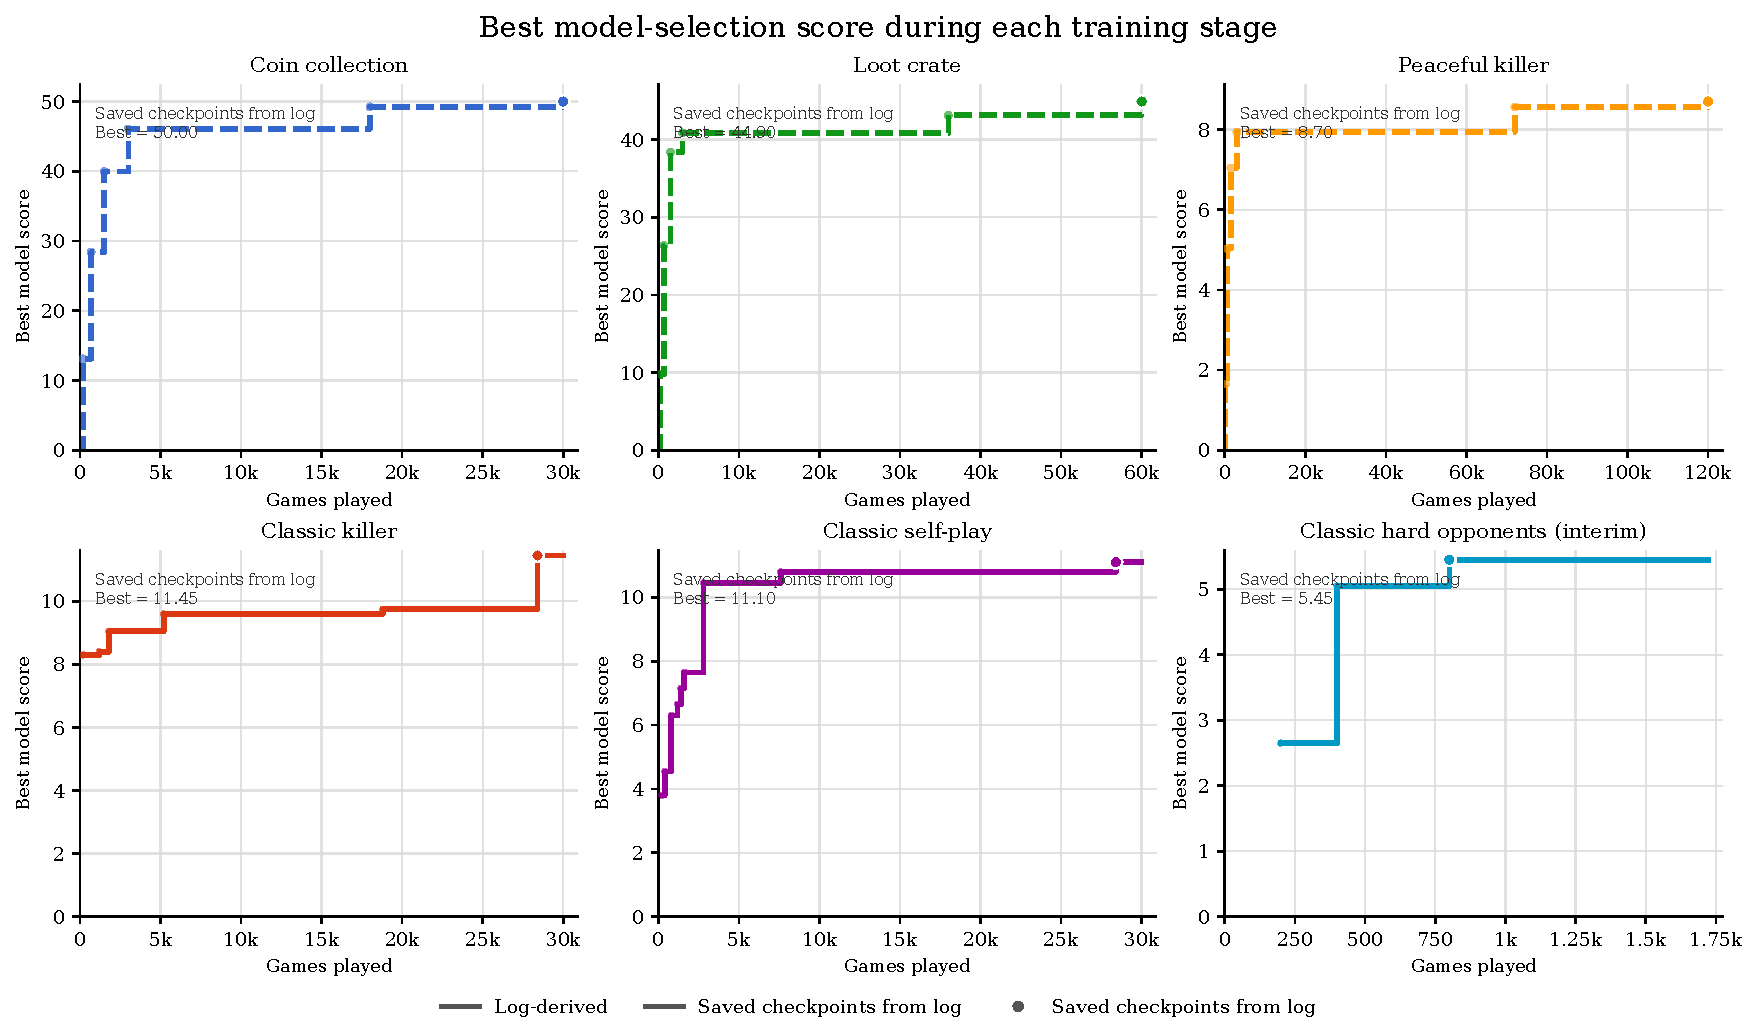
\includegraphics[width=\textwidth]{figures/best_model_score_by_stage.pdf}
\caption{Best model-selection score as a function of games played in each
training stage. The evaluations take place every 200 games, and the current best model is saved if its score improves.
The scores of the best models at each checkpoint are reported in
Table~\ref{tab:training-stage-results}.}
\label{fig:best-score-stages}
\end{figure}


\FloatBarrier

\subsection{Conclusion}
\section{Conclusion}

We developed and evaluated a different agents based on Double DQN, a dueling network architecture, engineered spatial and scalar features, action masking, and a staged training curriculum. 
The curriculum successfully decomposed the task into progressively harder objectives: the agent learned coin collection perfectly in \texttt{coin-heaven} and acquired effective crate-destruction behavior in \texttt{loot-crate}. 
In the competitive stages, it also learned to destroy crates, collect coins, and occasionally eliminate opponents while keeping self-destruction rates comparatively low.

In the case of the \texttt{ruehl\_base\_agent}, the agent struggled to achieve consistent success against hard opponents, highlighting the gap between performance in simplified training environments and competitive \texttt{classic} games.
In particular, the best model against hard opponents achieved a mean score of $3.95$ over 20 evaluation games, with a mean of $0.40$ opponent eliminations and no completed rounds.  
Thus, the agent learned meaningful bomb-use and survival-related behavior, but is unable to overcome the enemies counter-strategies consistently.

Possible next steps include evaluation over longer training periods, more systematic hyperparameter tuning, and training against a diverse population of opponents. These extensions would clarify which design choices contribute most strongly to performance and may improve robustness in the full competitive setting.


\FloatBarrier
\bibliographystyle{plainnat}
\bibliography{bib/references}

\end{document}
